%--------------------
% Packages
% -------------------
\documentclass[11pt,english]{article}
\usepackage{amsfonts}
\usepackage[left=2.5cm,top=2cm,right=2.5cm,bottom=3cm,bindingoffset=0cm]{geometry}
\usepackage{amsmath, amsthm, amssymb}
\usepackage{tikz}
\usetikzlibrary{calc}
\usetikzlibrary{decorations.pathreplacing,calligraphy}
\usepackage{fancyhdr}
%\usepackage{currfile}
\usepackage{nicefrac}
\usepackage{cite}
\usepackage{graphicx}
\usepackage{caption}
\usepackage{longtable}
\usepackage{rotating}
\usepackage{lscape}
\usepackage{booktabs}
\usepackage{float}
\usepackage{placeins}
\usepackage{setspace}
\usepackage[font=itshape]{quoting}
\onehalfspacing
\usepackage{mathrsfs}
\usepackage{tcolorbox}
\usepackage{xcolor}
\usepackage{subcaption}
\usepackage{float}
\usepackage[multiple]{footmisc}
\usepackage[T1]{fontenc}
\usepackage[sc]{mathpazo}
\usepackage{listings}
\usepackage{longtable}
\definecolor{cmured}{RGB}{175,30,45}
\definecolor{macroblue}{RGB}{56,108,176}
\usepackage[format=plain,
            labelfont=bf,
            textfont=]{caption}
\usepackage[colorlinks=true,citecolor=macroblue,linkcolor=macroblue,urlcolor=macroblue]{hyperref}
\usepackage{varioref}
\usepackage{chngcntr}
\usepackage{datetime}

\definecolor{darkgreen}{RGB}{30,175,88}
\definecolor{darkblue}{RGB}{30,118,175}
\definecolor{maroon}{rgb}{0.66,0,0}
\definecolor{darkgreen}{rgb}{0,0.69,0}

%Counters
\newtheorem{theorem}{Theorem}[section] 
\newtheorem{proposition}{Proposition}
\newtheorem{lemma}{Lemma}
\newtheorem{corollary}{Corollary}
\newtheorem{assumption}{Assumption}
\newtheorem{axiom}{Axiom}
\newtheorem{case}{Case}
\newtheorem{claim}{Claim}
\newtheorem{condition}{Condition}
\newtheorem{definition}{Definition}
\newtheorem{example}{Example}
\newtheorem{notation}{Notation}
\newtheorem{remark}{Remark}


\hypersetup{ 	
pdfsubject = {},
pdftitle = {TidyTuesday Week 1},
pdfauthor = {Pranay Gundam},
linkcolor= macroblue
}


\title{\textbf{TidyTuesday Week 1}}
\author{Pranay Gundam}


%-----------------------
% Begin document
%-----------------------
\begin{document}

\maketitle

\tableofcontents

\section{Weekly Summary}


\section{Date: 2025-01-02}
\noindent \textbf{Series ID: WPDILVA} 

\noindent This series is titled Discussion About Pandemics Index for Latvia and has a frequency of Quarterly. The units are Index and the seasonal adjustment is Not Seasonally Adjusted.The observation start date is 1996-01-01 and the observation end date is 2024-07-01.The popularity of this series is 1. \\ 

\noindent \textbf{Series ID: CCDIOA17140Q156N} 

\noindent This series is titled CredAbility Consumer Distress Index for Cincinnati-Middletown, OH-KY-IN (MSA) (DISCONTINUED) and has a frequency of Quarterly. The units are Percent and the seasonal adjustment is Not Seasonally Adjusted.The observation start date is 2005-01-01 and the observation end date is 2013-01-01.The popularity of this series is 0. \\ 

\subsection{Regression Tables and Plots}
\begin{center}
\begin{tabular}{lclc}
\toprule
\textbf{Dep. Variable:}       & value\_fred\_CCDIOA17140Q156N & \textbf{  R-squared:         } &     0.000   \\
\textbf{Model:}               &              OLS              & \textbf{  Adj. R-squared:    } &     0.000   \\
\textbf{Method:}              &         Least Squares         & \textbf{  F-statistic:       } &       nan   \\
\textbf{Date:}                &        Thu, 02 Jan 2025       & \textbf{  Prob (F-statistic):} &      nan    \\
\textbf{Time:}                &            10:10:29           & \textbf{  Log-Likelihood:    } &   -94.269   \\
\textbf{No. Observations:}    &                 33            & \textbf{  AIC:               } &     190.5   \\
\textbf{Df Residuals:}        &                 32            & \textbf{  BIC:               } &     192.0   \\
\textbf{Df Model:}            &                  0            & \textbf{                     } &             \\
\textbf{Covariance Type:}     &           nonrobust           & \textbf{                     } &             \\
\bottomrule
\end{tabular}
\begin{tabular}{lcccccc}
                              & \textbf{coef} & \textbf{std err} & \textbf{t} & \textbf{P$> |$t$|$} & \textbf{[0.025} & \textbf{0.975]}  \\
\midrule
\textbf{const}                &      71.4297  &        0.744     &    95.956  &         0.000        &       69.913    &       72.946     \\
\textbf{value\_fred\_WPDILVA} &            0  &            0     &       nan  &           nan        &            0    &            0     \\
\bottomrule
\end{tabular}
\begin{tabular}{lclc}
\textbf{Omnibus:}       & 10.222 & \textbf{  Durbin-Watson:     } &    0.253  \\
\textbf{Prob(Omnibus):} &  0.006 & \textbf{  Jarque-Bera (JB):  } &    2.567  \\
\textbf{Skew:}          &  0.159 & \textbf{  Prob(JB):          } &    0.277  \\
\textbf{Kurtosis:}      &  1.671 & \textbf{  Cond. No.          } &      inf  \\
\bottomrule
\end{tabular}
%\caption{OLS Regression Results}
\end{center}

Notes: \newline
 [1] Standard Errors assume that the covariance matrix of the errors is correctly specified. \newline
 [2] The smallest eigenvalue is      0. This might indicate that there are \newline
 strong multicollinearity problems or that the design matrix is singular.

\begin{figure}
\centering
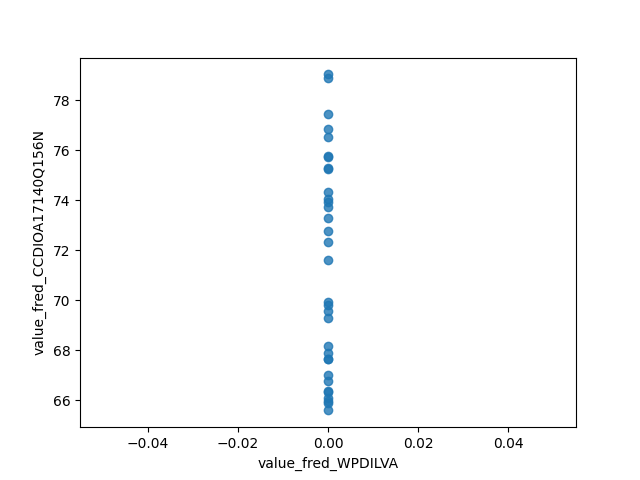
\includegraphics[scale = 0.9]{plots/plot_2025-01-02.png}
\caption{Regression Plot for 2025-01-02}
\end{figure}
\newpage

\include{tex_things/day_2025-01-03}
\include{tex_things/day_2025-01-04}
\include{tex_things/day_2025-01-05}
\section{Date: 2025-01-06}
\noindent \textbf{Series ID: PE5T17NE31163A647NCEN} 

\noindent This series is titled Estimate of Related Children Age 5-17 in Families in Poverty for Sherman County, NE and has a frequency of Annual. The units are Persons and the seasonal adjustment is Not Seasonally Adjusted.The observation start date is 1989-01-01 and the observation end date is 2023-01-01.The popularity of this series is 0. \\ 

\noindent \textbf{Series ID: NCOALLSRE1FRMACB} 

\noindent This series is titled Asset Quality Measures, Net Charge-Offs on All Loans and Leases, Secured by Real Estate, Single Family Residential Mortgages, Booked in Domestic Offices, All Commercial Banks and has a frequency of Quarterly. The units are Millions of Dollars and the seasonal adjustment is Not Seasonally Adjusted.The observation start date is 1991-01-01 and the observation end date is 2024-07-01.The popularity of this series is 2. \\ 

\subsection{Regression Tables and Plots}
\begin{center}
\begin{tabular}{lclc}
\toprule
\textbf{Dep. Variable:}                     & value\_fred\_NCOALLSRE1FRMACB & \textbf{  R-squared:         } &     0.009   \\
\textbf{Model:}                             &              OLS              & \textbf{  Adj. R-squared:    } &    -0.027   \\
\textbf{Method:}                            &         Least Squares         & \textbf{  F-statistic:       } &    0.2576   \\
\textbf{Date:}                              &        Mon, 06 Jan 2025       & \textbf{  Prob (F-statistic):} &    0.616    \\
\textbf{Time:}                              &            13:19:18           & \textbf{  Log-Likelihood:    } &   -276.39   \\
\textbf{No. Observations:}                  &                 29            & \textbf{  AIC:               } &     556.8   \\
\textbf{Df Residuals:}                      &                 27            & \textbf{  BIC:               } &     559.5   \\
\textbf{Df Model:}                          &                  1            & \textbf{                     } &             \\
\textbf{Covariance Type:}                   &           nonrobust           & \textbf{                     } &             \\
\bottomrule
\end{tabular}
\begin{tabular}{lcccccc}
                                            & \textbf{coef} & \textbf{std err} & \textbf{t} & \textbf{P$> |$t$|$} & \textbf{[0.025} & \textbf{0.975]}  \\
\midrule
\textbf{const}                              &    -329.7910  &     4436.181     &    -0.074  &         0.941        &    -9432.083    &     8772.501     \\
\textbf{value\_fred\_PE5T17NE31163A647NCEN} &      26.0933  &       51.412     &     0.508  &         0.616        &      -79.396    &      131.583     \\
\bottomrule
\end{tabular}
\begin{tabular}{lclc}
\textbf{Omnibus:}       & 20.243 & \textbf{  Durbin-Watson:     } &    0.266  \\
\textbf{Prob(Omnibus):} &  0.000 & \textbf{  Jarque-Bera (JB):  } &   24.859  \\
\textbf{Skew:}          &  1.891 & \textbf{  Prob(JB):          } & 4.00e-06  \\
\textbf{Kurtosis:}      &  5.504 & \textbf{  Cond. No.          } &     597.  \\
\bottomrule
\end{tabular}
%\caption{OLS Regression Results}
\end{center}

Notes: \newline
 [1] Standard Errors assume that the covariance matrix of the errors is correctly specified.

\begin{figure}
\centering
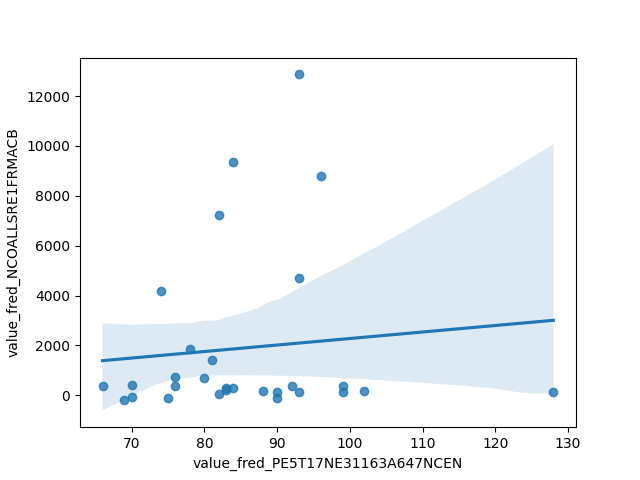
\includegraphics[scale = 0.9]{plots/plot_2025-01-06.png}
\caption{Regression Plot for 2025-01-06}
\end{figure}
\newpage

\section{Date: 2025-01-07}
\noindent \textbf{Series ID: MEANAGINE31A052NCEN} 

\noindent This series is titled Mean Adjusted Gross Income for Nebraska and has a frequency of Annual. The units are Dollars and the seasonal adjustment is Not Seasonally Adjusted.The observation start date is 1989-01-01 and the observation end date is 2022-01-01.The popularity of this series is 1. \\ 

\noindent \textbf{Series ID: RGDPTHJPA630NUPN} 

\noindent This series is titled Purchasing Power Parity Converted GDP Laspeyres per hour worked by employees for Japan and has a frequency of Annual. The units are 2005 International Dollars per Hour and the seasonal adjustment is Not Seasonally Adjusted.The observation start date is 1950-01-01 and the observation end date is 2010-01-01.The popularity of this series is 1. \\ 

\subsection{Regression Tables and Plots}
\begin{center}
\begin{tabular}{lclc}
\toprule
\textbf{Dep. Variable:}                   & value\_fred\_RGDPTHJPA630NUPN & \textbf{  R-squared:         } &     0.960   \\
\textbf{Model:}                           &              OLS              & \textbf{  Adj. R-squared:    } &     0.958   \\
\textbf{Method:}                          &         Least Squares         & \textbf{  F-statistic:       } &     484.1   \\
\textbf{Date:}                            &        Tue, 07 Jan 2025       & \textbf{  Prob (F-statistic):} &  1.73e-15   \\
\textbf{Time:}                            &            12:51:04           & \textbf{  Log-Likelihood:    } &   -24.588   \\
\textbf{No. Observations:}                &                 22            & \textbf{  AIC:               } &     53.18   \\
\textbf{Df Residuals:}                    &                 20            & \textbf{  BIC:               } &     55.36   \\
\textbf{Df Model:}                        &                  1            & \textbf{                     } &             \\
\textbf{Covariance Type:}                 &           nonrobust           & \textbf{                     } &             \\
\bottomrule
\end{tabular}
\begin{tabular}{lcccccc}
                                          & \textbf{coef} & \textbf{std err} & \textbf{t} & \textbf{P$> |$t$|$} & \textbf{[0.025} & \textbf{0.975]}  \\
\midrule
\textbf{const}                            &      14.9471  &        0.755     &    19.796  &         0.000        &       13.372    &       16.522     \\
\textbf{value\_fred\_MEANAGINE31A052NCEN} &       0.0004  &     1.72e-05     &    22.002  &         0.000        &        0.000    &        0.000     \\
\bottomrule
\end{tabular}
\begin{tabular}{lclc}
\textbf{Omnibus:}       &  5.134 & \textbf{  Durbin-Watson:     } &    0.758  \\
\textbf{Prob(Omnibus):} &  0.077 & \textbf{  Jarque-Bera (JB):  } &    3.967  \\
\textbf{Skew:}          & -1.040 & \textbf{  Prob(JB):          } &    0.138  \\
\textbf{Kurtosis:}      &  2.965 & \textbf{  Cond. No.          } & 2.00e+05  \\
\bottomrule
\end{tabular}
%\caption{OLS Regression Results}
\end{center}

Notes: \newline
 [1] Standard Errors assume that the covariance matrix of the errors is correctly specified. \newline
 [2] The condition number is large,  2e+05. This might indicate that there are \newline
 strong multicollinearity or other numerical problems.

\begin{figure}
\centering
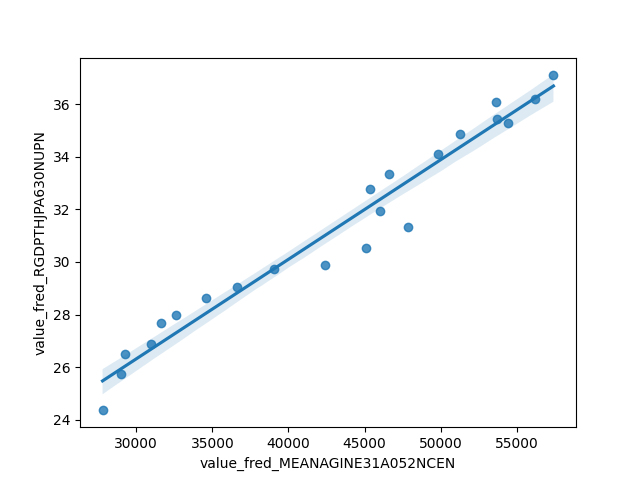
\includegraphics[scale = 0.9]{plots/plot_2025-01-07.png}
\caption{Regression Plot for 2025-01-07}
\end{figure}
\newpage

\section{Date: 2025-01-08}
\noindent \textbf{Series ID: ASTPIRQ027S} 

\noindent This series is titled All Sectors; Taxes on Production and Imports, Receivable (IMA), Transactions and has a frequency of Quarterly. The units are Millions of Dollars and the seasonal adjustment is Seasonally Adjusted Annual Rate.The observation start date is 1946-10-01 and the observation end date is 2024-07-01.The popularity of this series is 1. \\ 

\noindent \textbf{Series ID: O4243MM157SCEN} 

\noindent This series is titled Merchant Wholesalers, Except Manufacturers' Sales Branches and Offices: Nondurable Goods: Apparel, Piece Goods, and Notions Inventories and has a frequency of Monthly, End of Month. The units are Percent and the seasonal adjustment is Seasonally Adjusted.The observation start date is 1992-02-01 and the observation end date is 2024-11-01.The popularity of this series is 1. \\ 

\subsection{Regression Tables and Plots}
\begin{center}
\begin{tabular}{lclc}
\toprule
\textbf{Dep. Variable:}           & value\_fred\_O4243MM157SCEN & \textbf{  R-squared:         } &     0.012   \\
\textbf{Model:}                   &             OLS             & \textbf{  Adj. R-squared:    } &     0.004   \\
\textbf{Method:}                  &        Least Squares        & \textbf{  F-statistic:       } &     1.543   \\
\textbf{Date:}                    &       Wed, 08 Jan 2025      & \textbf{  Prob (F-statistic):} &    0.216    \\
\textbf{Time:}                    &           12:51:13          & \textbf{  Log-Likelihood:    } &   -268.13   \\
\textbf{No. Observations:}        &               130           & \textbf{  AIC:               } &     540.3   \\
\textbf{Df Residuals:}            &               128           & \textbf{  BIC:               } &     546.0   \\
\textbf{Df Model:}                &                 1           & \textbf{                     } &             \\
\textbf{Covariance Type:}         &          nonrobust          & \textbf{                     } &             \\
\bottomrule
\end{tabular}
\begin{tabular}{lcccccc}
                                  & \textbf{coef} & \textbf{std err} & \textbf{t} & \textbf{P$> |$t$|$} & \textbf{[0.025} & \textbf{0.975]}  \\
\midrule
\textbf{const}                    &       0.5960  &        0.467     &     1.277  &         0.204        &       -0.327    &        1.519     \\
\textbf{value\_fred\_ASTPIRQ027S} &   -5.093e-07  &      4.1e-07     &    -1.242  &         0.216        &    -1.32e-06    &     3.02e-07     \\
\bottomrule
\end{tabular}
\begin{tabular}{lclc}
\textbf{Omnibus:}       &  2.213 & \textbf{  Durbin-Watson:     } &    1.410  \\
\textbf{Prob(Omnibus):} &  0.331 & \textbf{  Jarque-Bera (JB):  } &    1.723  \\
\textbf{Skew:}          &  0.252 & \textbf{  Prob(JB):          } &    0.422  \\
\textbf{Kurtosis:}      &  3.253 & \textbf{  Cond. No.          } & 3.16e+06  \\
\bottomrule
\end{tabular}
%\caption{OLS Regression Results}
\end{center}

Notes: \newline
 [1] Standard Errors assume that the covariance matrix of the errors is correctly specified. \newline
 [2] The condition number is large, 3.16e+06. This might indicate that there are \newline
 strong multicollinearity or other numerical problems.

\begin{figure}
\centering
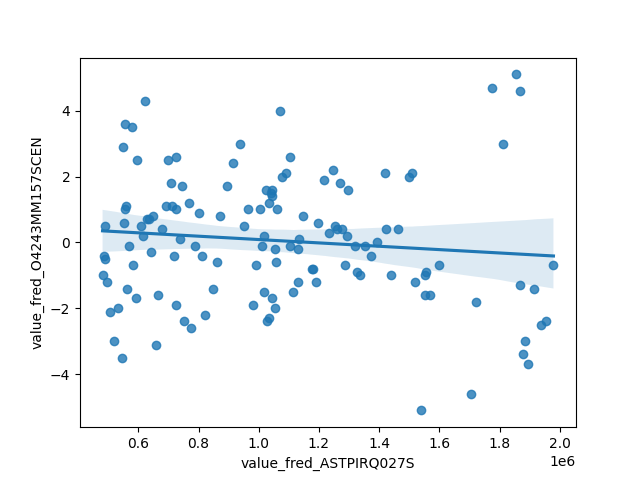
\includegraphics[scale = 0.9]{plots/plot_2025-01-08.png}
\caption{Regression Plot for 2025-01-08}
\end{figure}
\newpage


\end{document}
